\subsection{Mobile platform}
A way to overcome the reach problem in the previous mentioned solutions, could be a mobile platform where the manipulator will be placed on, so that the manipulator can be moved to reach any of the machines that the rotor has to go through to complete the work process. Usually having a mobile platform requires sensors which can give the platform a vision to move around within the work-cell\cite{doi:10.1177/1729881417718588}. Furthermore it usually would require that the platform is programmed by an expert, but in this article \cite{doi:10.1177/1729881417718588} they focus on making a more user friendly platform, so that the worker at the station can program and incorporate, the mobile platform to fit into a new work situation.\\

\subsection{A rail} 
A rail could also be another solution to extend the reach of the manipulator, by installing the manipulator on or under a rail so the manipulator can move back and fourth on a single axis or in a plane like a gantry crane. This solution will require two rails where one has to be installed on top of the other on a perpendicular axis\cite{FRUNS}.

\section{End-effector}

In this section the 3 most used gripper types being used in the industry, will be explained.

\subsection{Mechanical gripper}
The End-effector which is available for the group in this project is a pneumatic driven gripper. The gripper weighs 0.5 Kg (excluding gripper fingers). It has an operation pressure range from 3 to 7 Bar and the gripper claws are operated independently\cite{MWC}.The gripper in its neutral state is open, when air pressure is applied to the gripper it will close.\\
To control the gripper, solenoid actuated valves are used. To operate the valve a voltage is applied to the solenoid and the valve will move to an open position and let air flow towards the gripper.\\
The group can use the gripper by connecting the valve to the control box of the manipulator, then use the valve through the teach pendant.\\ 

\begin{figure}[H]
    \centering
    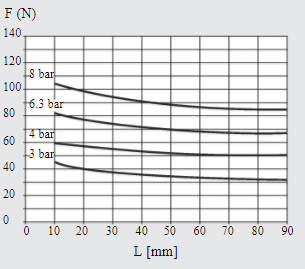
\includegraphics{TechnicalAnlysis/MWforcedia.PNG}
    \caption{This diagram shows the force object depending on the pressure and length of gripper fingers\cite{MWC}}
    \label{fig:Mvforce}
\end{figure}

\subsection{Suction / vacuum cup}
This kind of gripper is mostly used for pick and placement of non-ferrous materials, where only one surface is available to handle the material.\\ 
It functions by causing a vacuum inside the cups to hold onto.\\
This type of gripper is good for picking up objects, which are smooth, flat, and clean, and are less suitable for picking up objects with holes in it \cite{Gripper1}.\\

\subsection{Magnet gripper}
The magnetized end-effector is functioning much like the vacuum cups, where it only can hold on to a single surface on ferrous materials, instead of functioning by vacuum, it is using magnets to hold onto materials. The gripper is switching been on/off mode by pushing compressed air into the case, to push the magnet on or off see fig \cite{MagnetCite}.\\
This type of end-effector has the drawback that, if fast movements occur, there is a chance for the material to slip off its grip, this can also occur for the vacuum gripper\cite{Gripper2}.\\

\begin{figure}[H]
    \centering
    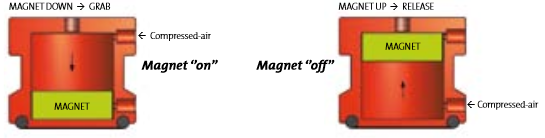
\includegraphics{TechnicalAnlysis/MagnetGripper.PNG}
    \caption{This figure shows how a basic Magnetic Gripper is turned on/off \cite{MagnetCite}}
    \label{fig:MagnetGrip}
\end{figure}

\subsection{Inflatable Gripper}
Inflatable bladder type grippers, functions like a balloon, which will be expanded once it is in the holding grip of the material, and is used to move items which requires fragile handling \cite{Gripper3}.\\

\section{Repeatability and accuracy}
When talking about Repeatability, it should not be confused with accuracy, though they are somewhat similar.\\
Repeatability is the factor of how high the spread rate is, which means a higher repeatability will cause the end-effector to reach closer to the same point on every repeat action.\\
Accuracy is the factor which tells us, how close the end-effector can be expected to reach the given position set by the user. This means a higher accuracy will lead to a diminished spread, compared to the position given in a space\cite{RepeatWhat}.\\

\begin{figure}[H]
    \centering
    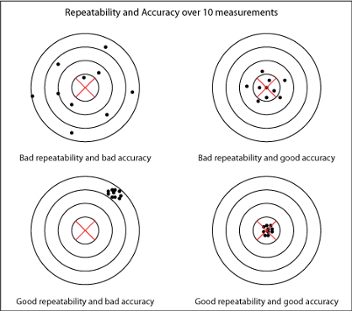
\includegraphics[width=.9\textwidth]{TechnicalAnlysis/RepeatTest.jpg}
    \caption{The difference between high/low repeatability and accuracy\cite{RepeatWhat}}
    \label{fig:Repeatability}
\end{figure}
